%%%%%%%%%%%%%%%%%%%%%%%%%%%%%%%%%%%%%%%%%%%%%%%%%%%%%%%%%%%%%%%%%%%%%%%%
%Desarrollo de un juego para Nintendo DS | Trabajo de Fin de Grado
% Escuela Politécnica Superior de la Universidad de Alicante
% Realizado por: Carla Maciá Díez
% Contacto: carlamd1997@hotmail.com / cmd23@alu.ua.es
%%%%%%%%%%%%%%%%%%%%%%%%%%%%%%%%%%%%%%%%%%%%%%%%%%%%%%%%%%%%%%%%%%%%%%%%

\chapter{Marco teórico}

\section{Nintendo DS} 

La \textbf{Nintendo DS} es una videoconsola portátil de la compañía de origen japonés \textbf{Nintendo}. Creada para suceder a la Game Boy Advance, se lanzó al mercado el \textbf{21 de noviembre de 2004 en Estados Unidos}, retrasándose su fecha de lanzamiento en \textbf{Japón al 2 de diciembre} y en\textbf{ Europa al 5 de marzo del año siguiente} con un \textbf{precio de 149.99€}. La consola original y sus versiones posteriores alcanzaron un total de \textbf{154,90 millones unidades vendidas} en todo el mundo y su videojuego más vendido fue el \textbf{New Super Mario Bros}, con un total de 30,80 millones de copias vendidas.

\vspace{0.5cm}

\begin{figure}[htbp]
\centering
  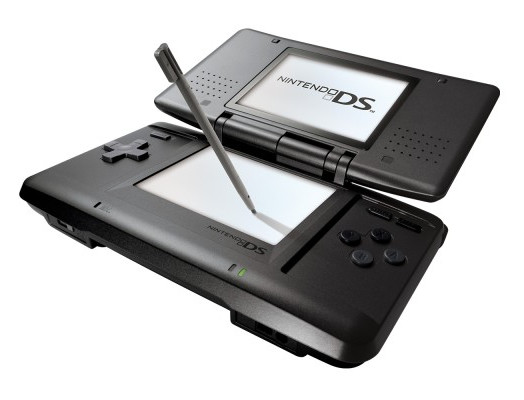
\includegraphics[width=0.4\textwidth]{archivos/nds.jpg}
  \caption{Nintendo DS}
  \textbf{Fuente:} \href{https://www.nintendo.co.uk/Nintendo-DS/Nintendo-DS-Family-Nintendo-UK-s-official-site-Nintendo-DS-Nintendo-DSi-Nintendo-DSi-XL-116380.html}{Nintendo}
  \label{fig:nds1}
\end{figure}

\vspace{0.5cm}

La consola consta de \textbf{ dos pantallas LCD} retroiluminadas con brillo ajustable, siendo una de ellas (la inferior) \textbf{ táctil}, un  \textbf{pad de direcciones},  \textbf{seis botones de acción} (A,B,X,Y, R y L) , \textbf{dos botones de control} (Start y Select) y un \textbf{micrófono}. En su interior posee \textbf{dos procesadores}, un \textbf{ARM946E-S} de 67 MHz que, en general, se encarga de la mayor parte del trabajo ejecutando los \textbf{juegos de NDS} y un \textbf{ARM7TDMI} de 33 MHz, que mueve los juegos de \textbf{GBA} y algunas funciones Wi-Fi. Profundizaremos en ambos procesadores más adelante.

\vspace{0.5cm}

Como curiosidad, las siglas DS significan \textbf{Developer's System} (Sistema de desarrolladores) ya que según la compañía, este sistema ofrece muchas herramientas para que los desarrolladores puedan innovar en sus creaciones. No obstante, también hicieron oficial que estas siglas también hacían referencia a \textbf{Dual Screen}, por su doble pantalla.

\vspace{1cm}

\subsection{Versiones}

Ahora que conocemos un poco más la Nintendo DS original, es importante que analicemos sus posteriores ediciones, ya que nuestro juego debe funcionar en cualquiera de ellas. Debemos conocer qué diferencias significativas existen y tenerlas en cuenta a la hora de desarrollar el juego. Así pues vamos a ir revisando la familia de consolas de Nintendo DS y conociendo sus principales cambios.

\vspace{1cm}

%\subsection{Nintendo DS}

%\begin{figure}[htbp]
%\centering
  %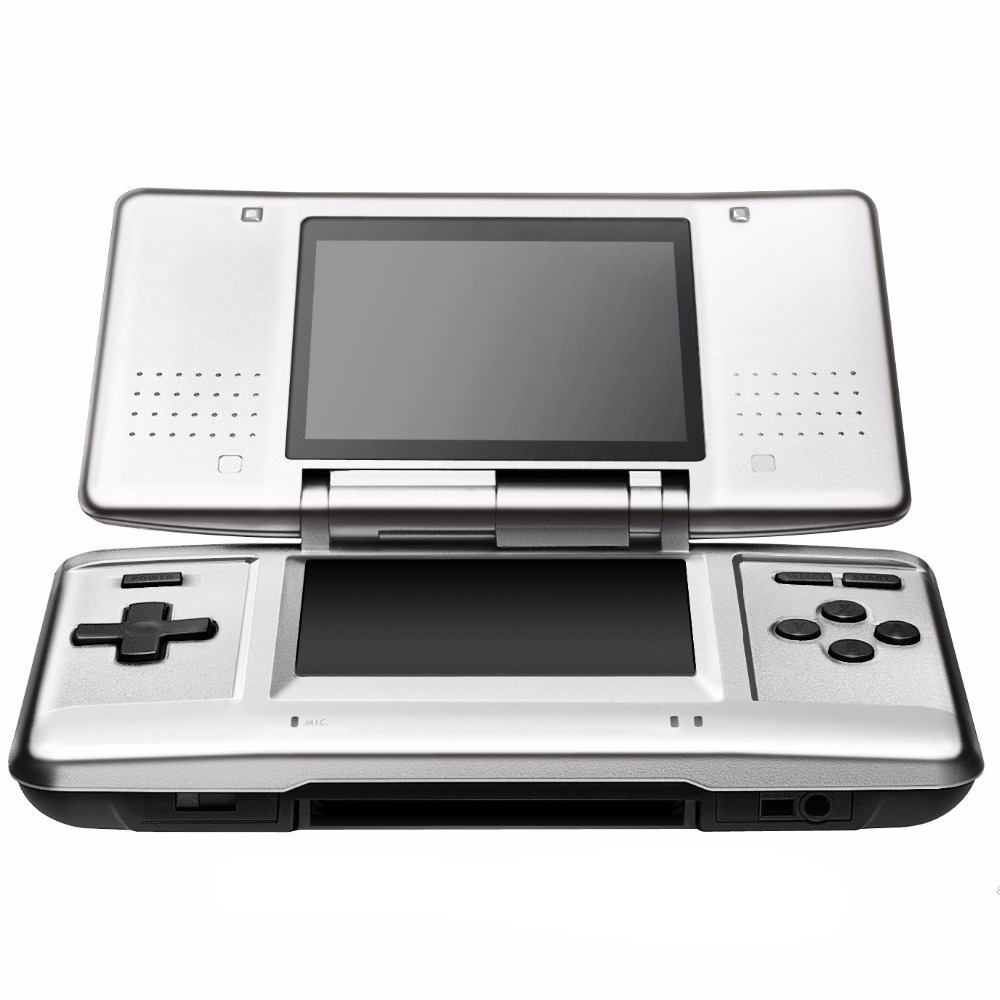
\includegraphics[width=0.3\textwidth]{archivos/nds2.jpg}
 % \caption{Nintendo DS}
  %\label{fig:nds2} %si cambio esto se irá la ref a la *??
%\end{figure}

\subsubsection{Nintendo DS Lite}

Fue creada en \textbf{2006} por Nintendo, es ligeramente \textbf{más pequeña} que su predecesora e incluía una \textbf{carcasa} más elegante. Algunos \textbf{botones} fueron \textbf{relocalizados} y añadía la función de poder elegir entre \textbf{4 niveles de brillo} a diferencia de la original, que solo podía ajustarse al mínimo o al máximo.

\vspace{0.5cm}

\begin{figure}[htbp]
\centering
  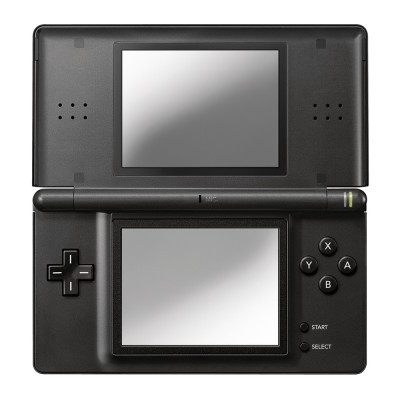
\includegraphics[width=0.3\textwidth]{archivos/ndslite.jpg}
  \caption{Nintendo DS Lite}
    \textbf{Fuente:} \href{https://www.nintendo.co.uk/Nintendo-DS/Nintendo-DS-Family-Nintendo-UK-s-official-site-Nintendo-DS-Nintendo-DSi-Nintendo-DSi-XL-116380.html}{Nintendo}
  \label{fig:ndslite}
\end{figure}

\vspace{1cm}

\subsubsection{Nintendo DSi}

Salió a la venta a finales de \textbf{2008 en Japón} y en \textbf{2009 en el restro del mundo} y se trata de una \textbf{revisión} del modelo de la Nintendo DS Lite. Si bien mantiene muchas características intactas, hay algunas otras que se deben destacar.

\vspace{0.5cm}

\begin{figure}[htbp]
\centering
  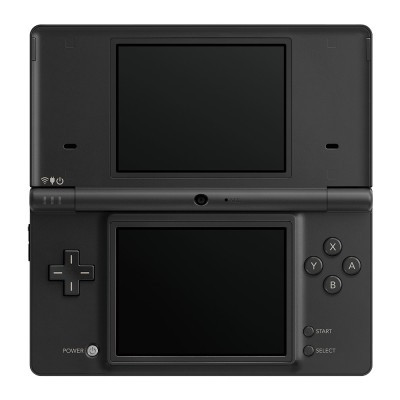
\includegraphics[width=0.3\textwidth]{archivos/ndsi.jpg}
  \caption{Nintendo DSi}
    \textbf{Fuente:} \href{https://www.nintendo.co.uk/Nintendo-DS/Nintendo-DS-Family-Nintendo-UK-s-official-site-Nintendo-DS-Nintendo-DSi-Nintendo-DSi-XL-116380.html}{Nintendo}
  \label{fig:ndsi}
\end{figure}

\vspace{0.5cm}

El primer cambio notable y que a mucha gente no le agradó, fue que \textbf{dejaba de ser compatible} con los juegos de \textbf{GBA}, pues ya no poseía ranura para los cartuchos. Introdujeron una \textbf{cámara delantera} y otra \textbf{trasera}, ambas de 0.3 megapíxeles, con las que podías hacer fotos y editarlas mediante un programa llamado \textbf{Cámara DSi} que venía instalado en la consola por defecto.  Poseía también una ranura para \textbf{tarjetas SD}, en las que podías guardar las fotos de la cámara así como los programas o juegos que descargases de la \textbf{Tienda Nintendo DSi}.

\vspace{0.5cm}

Por último, otras mejoras o diferencias frente a sus modelos originales son una \textbf{mejora de la calidad del audio}, \textbf{aumento} de la \textbf{memoria interna y RAM}, el procesador principal \textbf{ARM9} pasó a ser de 133 MHz (\textbf{aumentando su velocidad}), un \textbf{aumento} ligero del \textbf{tamaño de las pantallas} y \textbf{reducción} de la \textbf{duración de la batería} a 16 horas, siendo de 18 horas y media las originales.

\vspace{0.5cm}

El \textbf{menú principal} de la consola es completamente distinto al de la DS original, pasando a ser bastante \textbf{más personalizable} y con una gran variedad de programas, los cuales algunos de ellos se mantenían desde la DS como el \textbf{Picto-Chat} o la \textbf{Descarga DS}.

\vspace{0.5cm}

\begin{figure}[htbp]
\centering
  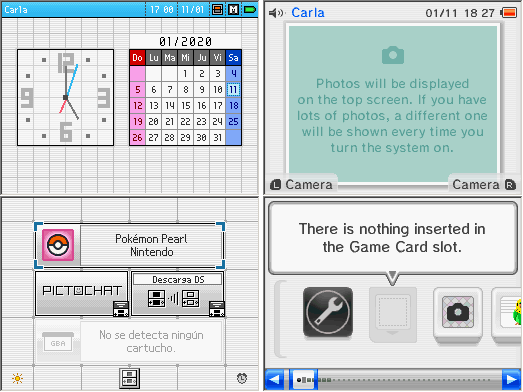
\includegraphics[width=0.6\textwidth]{archivos/nds-ndsi-menu.png}
  \caption{Menú de Nintendo DS (izquierda) frente al de Nintendo DSi (derecha)}
  \label{fig:menu-comparacion} %si cambio esto se irá la ref a la *??
\end{figure}

\vspace{0.5cm}

Fué la primera consola portátil en tener \textbf{bloqueo regional}, no permitiendo que juegos desarrollados en países extranjeros se ejecutasen en la consola si esta era originaria del mismo país.

\vspace{1cm}

\subsubsection{Nintendo DSi XL}

Se trata de un modelo adicional de NDSi que salió a la venta en \textbf{Japón en 2009}, donde originalmente se bautizó como Nintendo DSi LL, llegando a \textbf{España en 2010} donde pasó a llamarse Nintendo DSi XL.

\vspace{0.5cm}

\begin{figure}[htbp]
\centering
  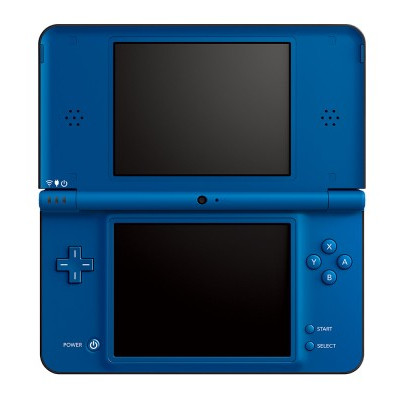
\includegraphics[width=0.3\textwidth]{archivos/ndsixl.jpg}
  \caption{Nintendo DSi XL}
    \textbf{Fuente:} \href{https://www.nintendo.co.uk/Nintendo-DS/Nintendo-DS-Family-Nintendo-UK-s-official-site-Nintendo-DS-Nintendo-DSi-Nintendo-DSi-XL-116380.html}{Nintendo}
  \label{fig:ndsixl} %si cambio esto se irá la ref a la *??
\end{figure}

\vspace{0.5cm}

El principal cambio destacable es el considerable aumento del tamaño de la consola como consecuencia del \textbf{aumento del tamaño de las pantallas} (estas tienen aproximadamente \textbf{una pulgada más} comparadas con la NDSi). En general es una consola perfecta para aquellos que tengan alguna discapacidad visual o les sea difícil o incómodo jugar con las anteriores por su tamaño.

\vspace{1cm}

\subsection{Especificaciones}

En esta sección vamos a conocer los detalles técnicos de la consola y profundizar en los más interesantes para poder entender qué la compone. Podemos ver a continuación una tabla a modo de resumen.
\clearpage

\begin{table}[htbp]

\centering

\begin{tabular}{|l|l|lll}

\cline{1-2}

\textbf{CPU}                & \begin{tabular}[c]{@{}l@{}}ARM946E-S 32bit RISC CPU\\ ARM7TDMI 32bit RISC CPU\end{tabular} &  &  &  \\ \cline{1-2}

\textbf{Velocidad de reloj} & \begin{tabular}[c]{@{}l@{}}(ARM9) 66MHz\\ (ARM7) 33MHz (16MHz en modo GBA)\end{tabular}    &  &  &  \\ \cline{1-2}

\textbf{RAM}                & 4096KB                                                                                     &  &  &  \\ \cline{1-2}

\textbf{VRAM}               & 656KB                                                                                      &  &  &  \\ \cline{1-2}

\textbf{Pantalla}           & 2 pantallas LCD (256x192 px, 3"). Una de ellas táctil.                                                           &  &  &  \\ \cline{1-2}

\textbf{Paleta de colores}  & 18-bit (262144 colores)                                                                    &  &  &  \\ \cline{1-2}

\textbf{Sonido}             & 16 canales de sonido estéreo                                                               &  &  &  \\ \cline{1-2}

\textbf{Comunicación}       & Wifi IEEE 802.11b                                                                          &  &  &  \\ \cline{1-2}

\textbf{Alimentación}       & Batería recargable de ion de litio 850mAh                                                  &  &  &  \\ \cline{1-2}

\textbf{Peso}               & 275g                                                                                       &  &  &  \\ \cline{1-2}

\textbf{Dimensiones}        & 148.7mm × 84.7mm × 28.9mm                                                                  &  &  &  \\ \cline{1-2}

\end{tabular}
\caption{Especificaciones técnicas de la NDS}
\end{table}

Para profundizar más acerca de los procesadores de la consola, su memoria de vídeo, zonas hardware específicas para gráficos, sonido y ROM, visita el \hyperref[anexo]{\textbf{Anexo I}}.

\vspace{1cm}


\section{Estudio de mercado}

Si bien la NDS fue una consola revolucionaria por su gran número de ventas así como el éxito de sus grandes títulos, hoy en día ya no se producen juegos para ésta, pues ha sido \textbf{sucedida por la 3DS}. Es por esto que el mercado a día de hoy se reduce a fanáticos que desean comprar en buen estado estos juegos y lo hacen mediante la venta de \textbf{segunda mano}.

\vspace{0.5cm}

No obstante, existe la llamada \textbf{\textit{Scene}}, conformada por los programadores e informáticos que desarrollan \textbf{aplicaciones y juegos no oficiales} para sistemas como es la NDS entre muchas otras. La existencia de este tipo de comunidades son muy buenas ya que gracias a foros o \textit{hashtags} como el de \#dsdev en Twitter puedes llegar a más público, haciendo que quizás se interesen por tu proyecto.

\vspace{1cm}

\section{Algoritmo de reconocimiento de escritura}

%LINKS: COMENTADOS

%http://cravesoft.free.fr/PAlibDocEng/html/group___reco.html#ga925cec3c4c9e826e8c07ee5a2366feb

%https://github.com/jichu4n/palm-os-sdk

%https://riunet.upv.es/bitstream/handle/10251/11576/memoria.pdf?sequence=1

%https://devkitpro.org/wiki/PAlib

%https://azydream.tistory.com/55

%https://github.com/atgreen/RTEMS/blob/master/c/src/lib/libbsp/arm/nds/touchscreen/reco.c

%https://es.wikipedia.org/wiki/Graffiti_(Palm_OS)

%http://patft.uspto.gov/netacgi/nph-Parser?Sect1=PTO1&Sect2=HITOFF&d=PALL&p=1&u=%2Fnetahtml%2FPTO%2Fsrchnum.htm&r=1&f=G&l=50&s1=5596656.PN.&OS=PN/5596656&RS=PN/5596656                  o                 https://patents.google.com/patent/US5596656

Algo esencial que necesitaremos para llevar a cabo este proyecto es un \textbf{algoritmo} que nos permita \textbf{reconocer el patrón que dibuje el usuario} en la pantalla táctil de entre unos que nosotros tengamos definidos. 

\vspace{0.5cm}

El desarrollo de un \textit{software} de estas características es sin duda algo que puede hacer que algunos desarrolladores se lleven las manos a la cabeza. Si bien es cierto que a día de hoy existen gran número de programas de pago o incluso integrados en nuestros teléfonos y ordenadores que son capaces de distinguir caracteres dibujados por usuarios, hay muy pocos de ellos de código abierto. Por suerte, tenemos un ejemplo de un \textit{software} así en el contexto que nos interesa.

\vspace{0.5cm}

Para el desarrollo en NDS existía una librería llamada \textbf{PAlib} que surgió en los primeros años de desarrollo \textit{homebrew} cuyo objetivo, al igual que \textbf{libnds}, era facilitar las tareas al programador. No obstante, a pesar de haber sido bien acogida por los usuarios por su sencillez y fácil uso, los encargados de mantener el conjunto de librerías y herramientas de \textbf{devkitPro} afirmaban que esta librería estaba \textbf{mal diseñada y provocaba serios fallos} en la consola tales como corrupciones de la tarjeta SD. Es por ello que devkitPro, del cual hablaremos más adelante, dejó de dar soporte a esta librería\footnote{https://devkitpro.org/wiki/PAlib} y ésta tras un tiempo esta cerró su página web y dejó de actualizarse. A día de hoy, parte de su documentación y código fuente siguen publicados en internet gracias a usuarios que lograron recuperarlas del archivo.

\vspace{0.5cm}

Lo que nos interesa a nosotros de esta librería es precisamente que implementó un \textbf{algoritmo de reconocimiento de escritura manuscrita} similar a otro más conocido como es \textbf{Graffiti de Palm}, pues en ambos la forma de dibujar los caracteres es la misma. Así pues, vamos a comprender a continuación cómo solucionan el problema ambos algoritmos.

\vspace{0.5cm}

\subsubsection{Graffiti de PAlib}

Como hemos comentado, este algoritmo de PAlib nos da como resultado el carácter al que más se parezca el dibujado por el usuario. Los trazos y sus respectivos carácteres son los mostrados en la siguiente figura, donde como podemos ver, no hay números ni algunos caracteres especiales como la 'ñ'. No obstante, esto es compensado con la posibilidad de poder incorporar \textbf{nuestros propios trazos}. 

\vspace{0.5cm}

\begin{figure}[htbp]
\centering
  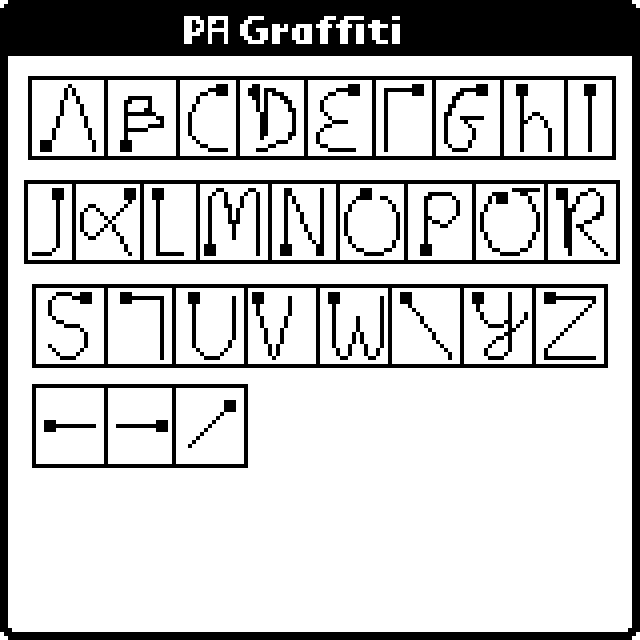
\includegraphics[width=0.3\textwidth]{archivos/pagraffiti.png}
  \caption{Caracteres y su trazo correspondiente de PA Graffiti}
  \textbf{Fuente:} \href{https://web.archive.org/web/20070708175646/http://www.palib.info/Reco/PAGraffiti.gif}{Documentación de PAlib (Recuperada del archivo)}
  \label{fig:pagraffiti}
\end{figure}

\vspace{0.5cm}

El algoritmo funciona de la siguiente manera: 

\vspace{0.5cm}

\begin{itemize}
 \item Guarda en un array cada par de coordenadas (x1,y1), ... , (xn,yn) que conforman el \textbf{trazo} introducido por el usuario.
 
 \item De toda esa lista de puntos, escoge \textbf{17} muestras para computarlas. 
 
 \item Calcula el \textbf{ángulo entre cada par de puntos} y le \textbf{asigna un carácter} dependiendo del rango en el que caiga dicho ángulo.
 
 \item \textbf{Compila todos los caracteres} de los ángulos calculados y genera una cadena de 16 caracteres que define dicho trazo.
 
 \item Busca dentro de unos trazos que ya tiene definidos, aquella \textbf{cadena de caracteres} que sea \textbf{más parecida} a la introducida por el usuario.
\end{itemize}

\vspace{0.5cm}

Como observamos, lo que básicamente hace el algoritmo es \textbf{caracterizar la línea con una cadena de caracteres} sirviendose del ángulo que forman los puntos de esta misma. Una vez calcula el ángulo que forman dos puntos, para saber qué caracter asignarle se vale de una circunferencia la cual está dividida en \textbf{32 rangos} como se ven en la siguiente figura.

\vspace{0.5cm}

\begin{figure}[htbp]
\centering
  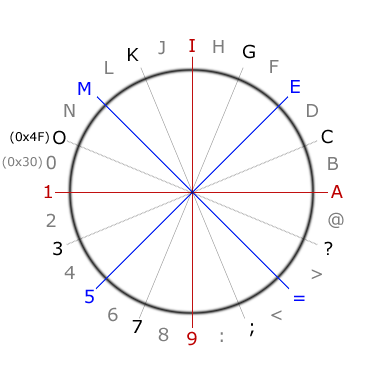
\includegraphics[width=0.5\textwidth]{archivos/recocircle.png}
  \caption{Correspondencia entre caracteres y los 32 rangos de ángulos.}
  \textbf{Fuente:} \href{https://azydream.tistory.com/55}{azyDream}
  \label{fig:recocircle}
\end{figure}

\vspace{0.5cm}

Así pues, un carácter como por ejemplo la letra 'i' equivaldría a la cadena '9999999999999999', pues al dibujarse completamente en vertical desde arriba hacia abajo todos los ángulos calculados caerían en el rango que equivale al 9.

\vspace{0.5cm}

En la figura siguiente veríamos un ejemplo de cuál sería la cadena asignada al trazo mostrado en blanco. Las líneas azules representan los 17 puntos de muestra. Como se ve, los primeros caracteres del trazo son A, pues el ángulo entre puntos es de 0 grados y conforme el trazo va descendiendo se le van asignando las letras de los rangos consecuentes.

\vspace{0.5cm}

\begin{figure}[htbp]
\centering
  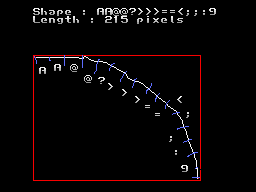
\includegraphics[width=0.5\textwidth]{archivos/recoex.png}
  \caption{Ejemplo de asignación de una cadena de caracteres a un trazo.}
  \textbf{Fuente:} \href{https://azydream.tistory.com/55}{azyDream}
  \label{fig:recoex}
\end{figure}


\vspace{0.5cm}

Esta forma de trabajar del algoritmo es lo que permite que puedas \textbf{introducir tus propios diseños de forma sencilla para el programador}, pues solo tienes que dibujar el patrón que deseas en un proyecto a parte y haciendo llamadas a las funciones de crear una forma te devolverían una cadena que identifica dicho trazo. De hecho, el algoritmo te da la posibilidad de analizar formas en base a unas que tiene predefinidas o las tuyas propias.

\vspace{0.5cm}

\subsubsection{Graffiti de Palm}

\textbf{Graffiti} es un \textit{software} de reconocimiento de escritura manuscrita desarrollado por el ingeniero informático \textbf{Jeff Hawkins} en \textbf{Palm} para las \textbf{PDAs} con sistema operativo PalmOS. Dicho \textit{software} crea una ligera modificación y simplificación de los carácteres alfabéticos, como podemos ver en la siguiente figura, para que puedan ser dibujados con un lápiz táctil sobre una pantalla y sin levantarlo hasta completar el trazo.

\clearpage


\begin{figure}[htbp]
\centering
  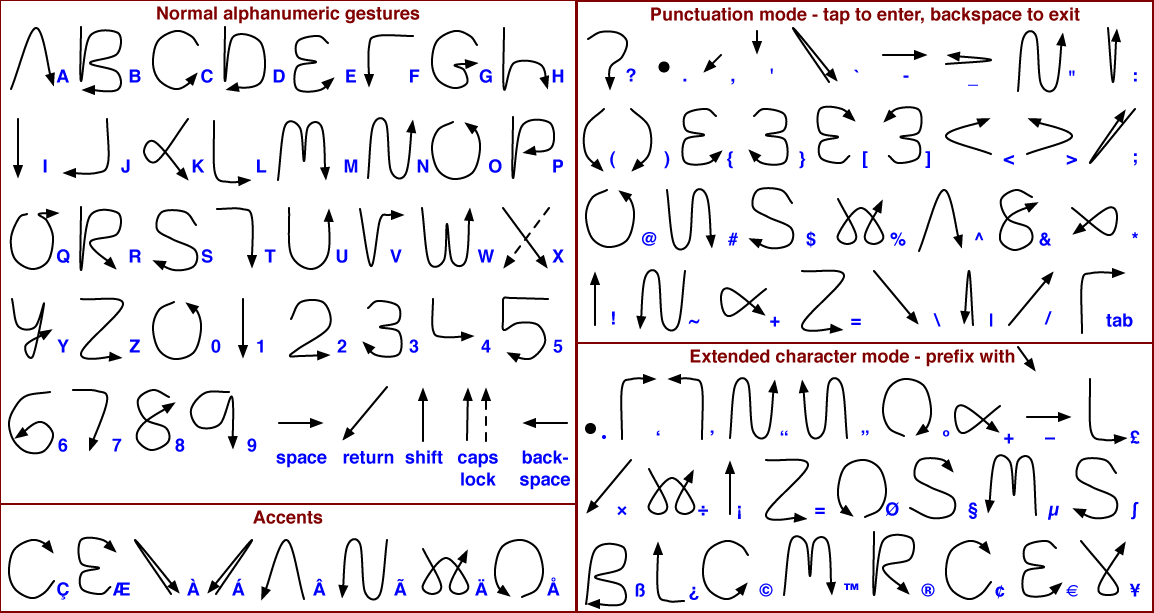
\includegraphics[width=0.6\textwidth]{archivos/palm_gestures.png}
  \caption{Gestos usados en PalmOS para definir los distintos caracteres}
\textbf{Fuente:} \href{https://es.wikipedia.org/wiki/Graffiti_(Palm_OS)#/media/Archivo:Palm_Graffiti_gestures.png}{IMewbot}
  \label{fig:palm_gestures}
\end{figure}

\vspace{0.5cm}

No obstante, Graffiti tuvo que ser \textbf{retirado y más tarde sustituido} por una nueva versión de este ya que la compañía \textbf{Xerox demandó a Palm} porque su \textit{software} de reconocimiento de escritura violaba la patente de Xerox sobre \textbf{tecnología Unistrokes}. Esto fue así porque Palm consiguió una demo de dicha tecnología antes de desarrollar su propio sistema.

\vspace{0.5cm}

Esto es importante comentarlo, pues a continuación explicaremos cómo funciona el algoritmo de la tecnología Unistrokes tal y como está reflejado en la pantente USPTO nº 5596656\footnote{https://patents.google.com/patent/US5596656}, pero debemos  tener en cuenta que la primera versión de Graffiti funciona de la misma manera.

\vspace{0.5cm}

Así pues, vamos a describir brevemente lo que hace el algoritmo para identificar el trazo:

\vspace{0.5cm}

\begin{itemize}
 \item Guardar en una lista ordenada cada par de coordenadas (x1,y1), . . . , (xn,yn) que conforman el \textbf{trazo}.
 \item \textbf{Filtrar dicha lista} para eliminar el posible ruido y suavizar así el trazo para facilitar el cálculo.
 \item Comprobar si se trata de una \textbf{línea recta} y, si es así, calcular la pendiente de esta. Usar esa pendiente para comprobar los caracteres que se generan con una línea, como por ejemplo i, 1, espaciado... Y terminar la búsqueda.
 \item Si no se trata de una línea recta, \textbf{normalizar} el trazo para que quepa en una caja cuadrada y calcular las siguientes características:
 
 \end{itemize}
 
 El \textbf{desplazamiento en el eje x} entre el origen y el final
  \begin{equation}
dx=xn-x1
\end{equation}

 El \textbf{desplazamiento en el eje y} entre el origen y el final
  \begin{equation}
dy=yn-y1
\end{equation}

El \textbf{desplazamiento entre el origen y el punto medio del trazo en el eje x}
\begin{equation}
 dx_{x1-xn/2}=x(n/2)-x1
\end{equation}

El \textbf{desplazamiento entre el origen y el punto medio del trazo en el eje y}
\begin{equation}
dy _{y1-yn/2}=y(n/2)-y1
\end{equation}

La \textbf{suma de las longitudes} de las líneas que unen cada punto con su predecesor \textbf{proyectado en el eje x}
\begin{equation}
lengthxtot = length_x(x1,x2) + length_x(x2,x3) + ... + length_x(xn-1,xn)
\end{equation}

La \textbf{suma de las longitudes} de las líneas que unen cada punto con su predecesor \textbf{proyectado en el eje y}
\begin{equation}
lengthytot = length_y(y1,y2) + length_y(y2,y3) + ... + length_y(yn-1,yn)
\end{equation}


\begin{itemize}
 \item Calculadas estas características, elegir el carácter que más se parece de una \textbf{tabla} como la siguiente:
\end{itemize}

\begin{table}[hbtp]
\centering
\begin{tabular}{c|c|c|c|c|c|c|}
\cline{2-7}
\multicolumn{1}{l|}{}           & dx        & dy        & dx(x1-xn/2) & dy(y1-yn/2) & length x tot & length y tot \\ \hline
\multicolumn{1}{|c|}{a}         & 0.0       & -1.0      & 0.0         & -0.5        & 0.0          & 1.0          \\ \hline
\multicolumn{1}{|c|}{b}         & 0.0       & 1.0       & 1.0         & 0.5         & 2.0          & 1.0          \\ \hline
\multicolumn{1}{|c|}{c}         & 0.0       & -1.0      & -1.0        & -0.5        & 2.0          & 1.0          \\ \hline
\multicolumn{1}{|c|}{d}         & 0.0       & 1.0       & -1.0        & 0.5         & 2.0          & 1.0          \\ \hline
\multicolumn{1}{|c|}{e}         & -1.0      & 0.0       & -0.5        & 0.0         & 1.0          & 0.0          \\ \hline
\multicolumn{1}{|c|}{{[}...{]}} & {[}...{]} & {[}...{]} & {[}...{]}   & {[}...{]}   & {[}...{]}    & {[}...{]}    \\ \hline
\end{tabular}
\caption{Datos de cada letra estudiados.}
\label{table:tablepalm}
\end{table}

\begin{itemize}
 \item Si el resultado es una U o una O, determinar si el trazo gira en el \textbf{sentido horario o antihorario} para afirmar si es una U o una O respectivamente.
\end{itemize}

\vspace{0.5cm}

Como podemos ver, el algoritmo calcula una serie de \textbf{valores que caracterizan la línea} y los compara con los que han estimado para los distintos caracteres que pueden dibujar. No obstante, debemos detenernos a entender dos de ellos pues son los que más confusión pueden provocar: lengthxtot y lengthytot.

\vspace{0.5cm}

Tal y como se explicaba anteriormente, este valor representa para cada eje, la suma de las longitudes de unas línea simaginarias desde un punto hasta su predecesor. Es importante no confundir este concepto con la distancia del punto inicial al final, pues si bien pueden coincidir en algunos casos, no significan lo mismo. Por ejemplo, imaginemos un trazo conformado por 3 puntos completamente colocados en vertical y separados en una unidad. En este caso, ambos valores serían iguales, 3, pero si el trazo lo modificamos para que tenga un cuarto punto inferior al tercero, ahora la longitud sería mayor a 3 y la distancia menor a tres, pues habríamos añadido un segmento más en el caso de la longitud y por el contrario, la distancia entre el punto inicial y final ahora es menor.

\vspace{0.5cm}

La siguiente figura muestra un ejemplo gráfico de cómo se representa estos valores:

\vspace{0.5cm}

\begin{figure}[htbp]
\centering
  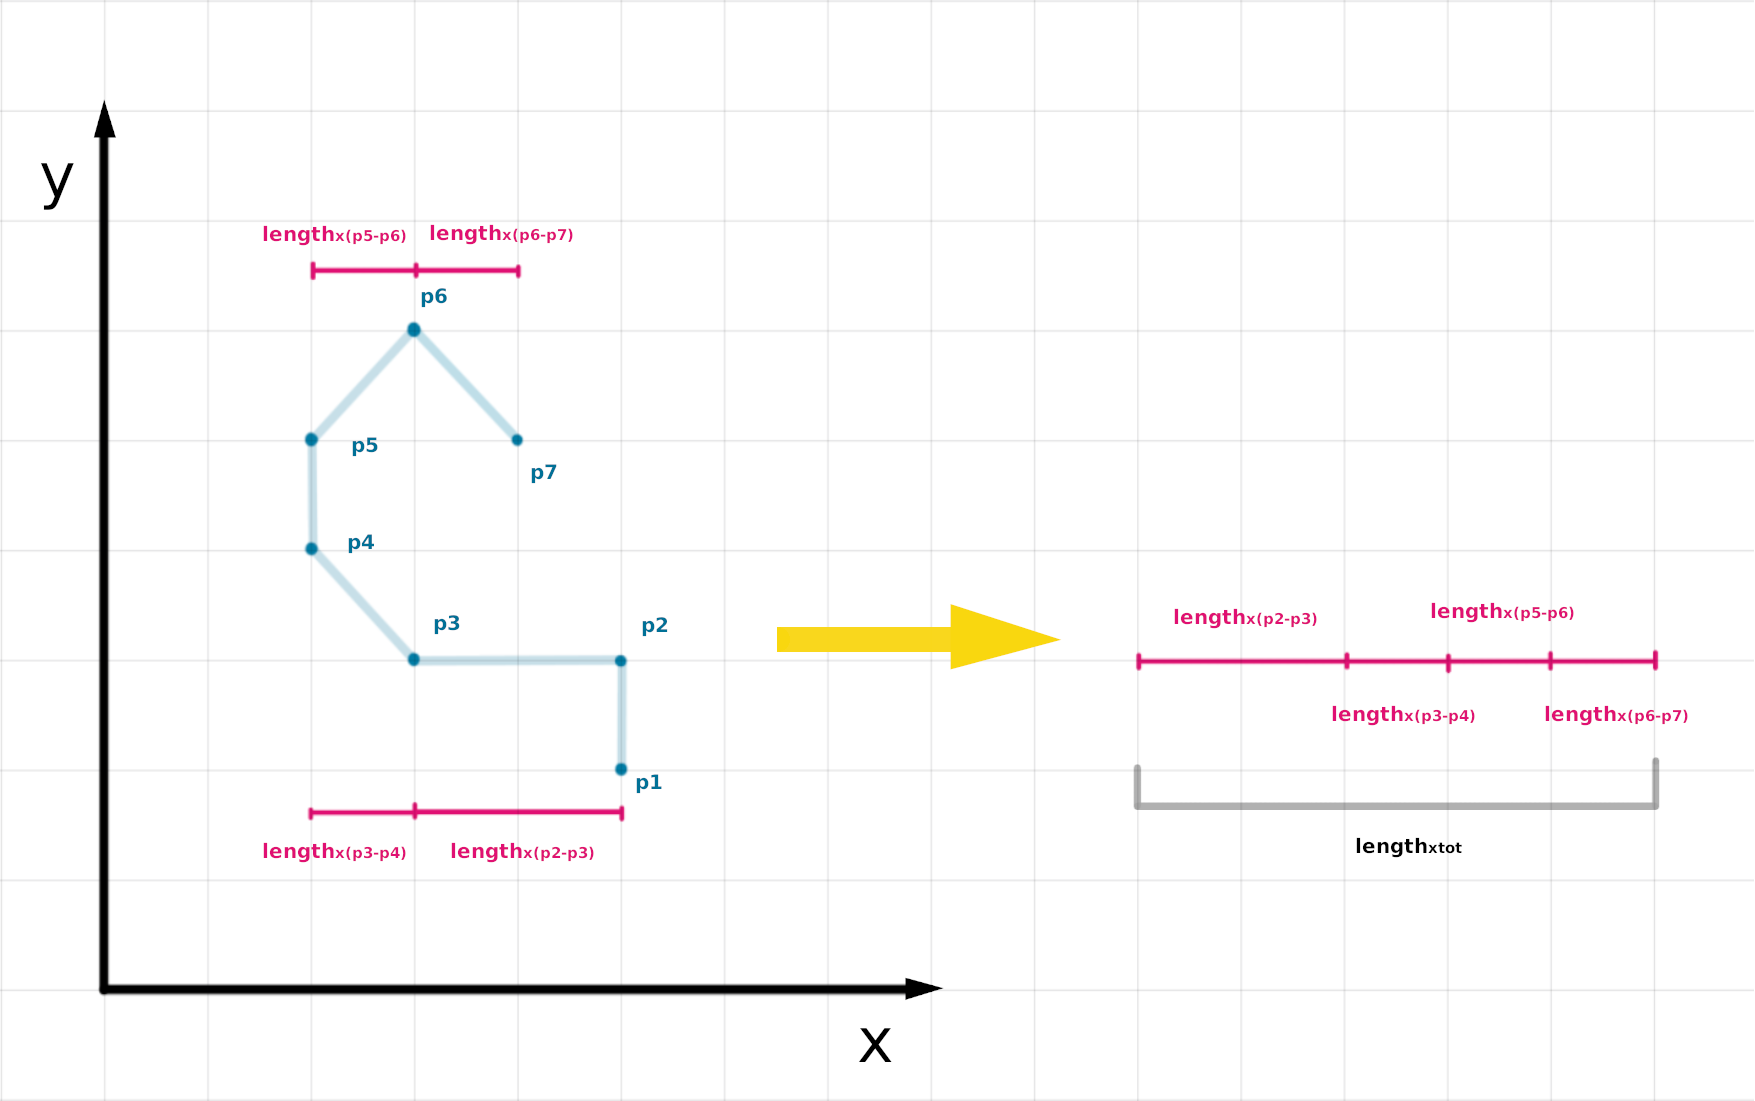
\includegraphics[width=0.8\textwidth]{archivos/vertline_x.png}
  \caption{Ejemplo gráfico del cálculo de la longitud total en el eje x}
  \label{fig:vertline_x}
\end{figure}

\clearpage

\begin{figure}[htbp]
\centering
  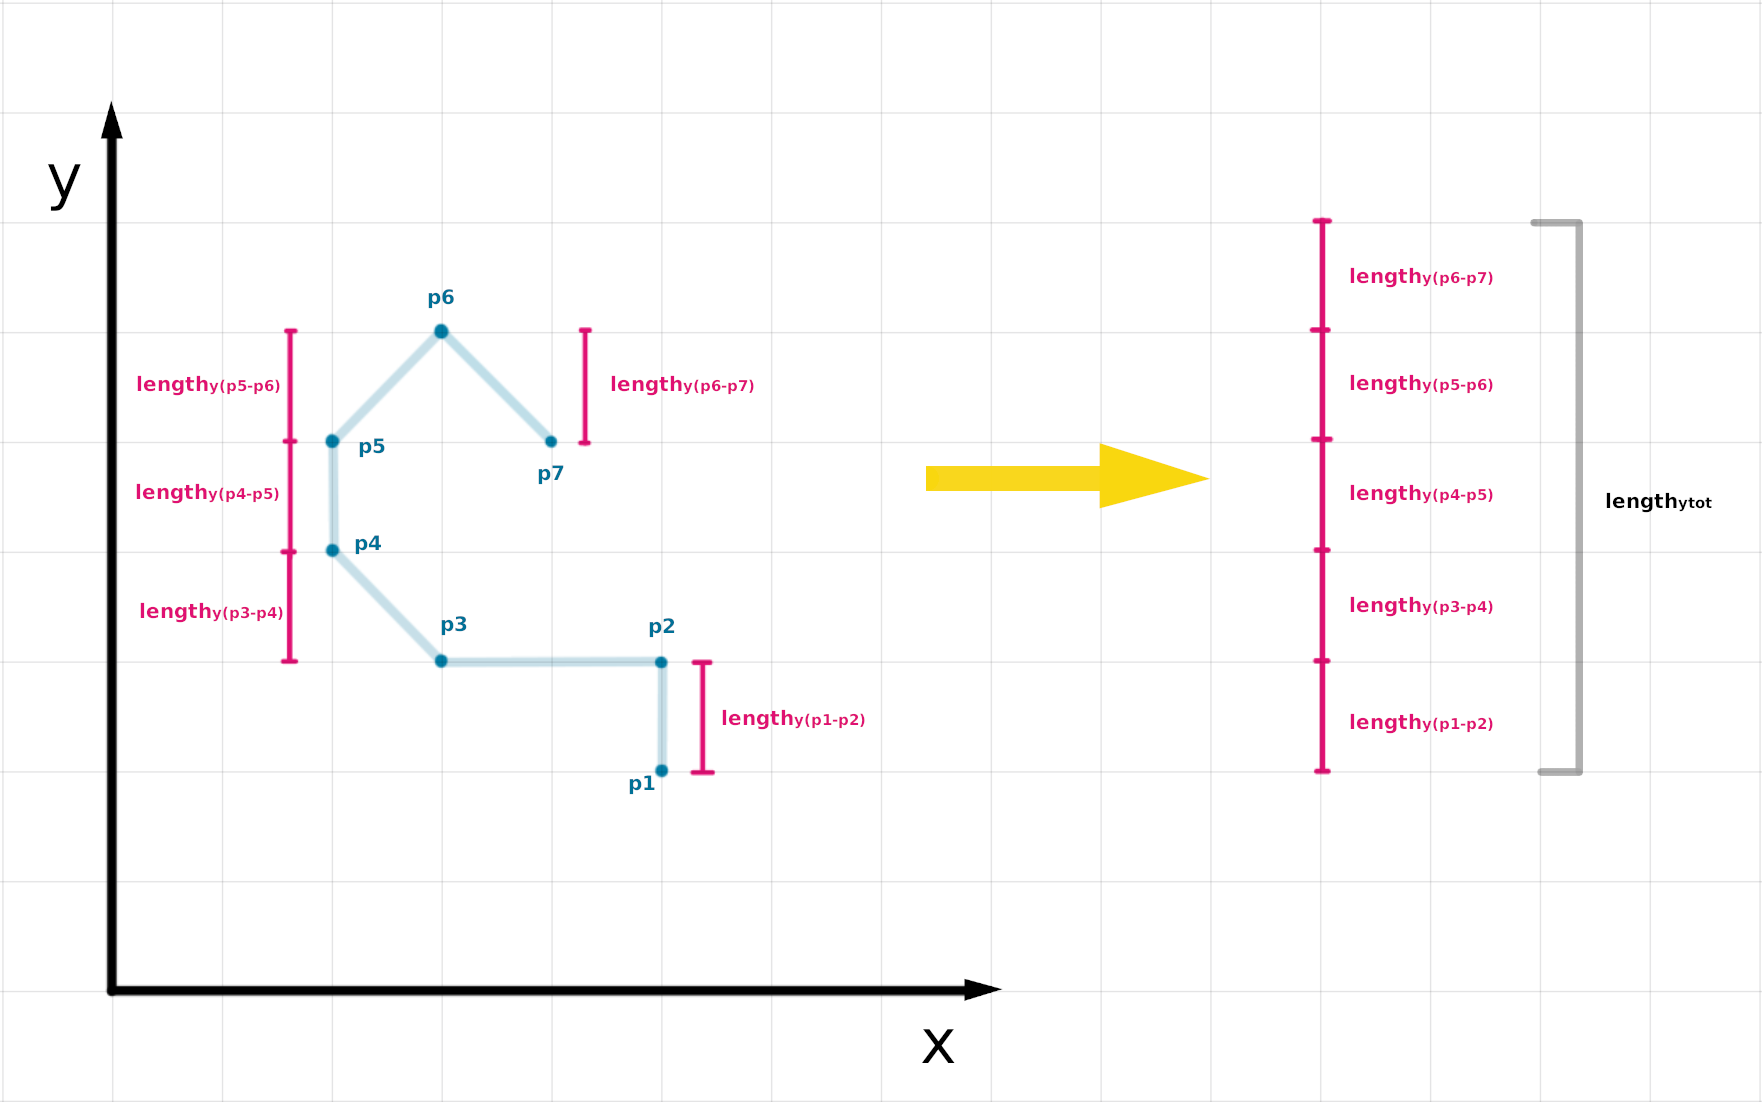
\includegraphics[width=0.8\textwidth]{archivos/vertline_y.png}
  \caption{Ejemplo gráfico del cálculo de la longitud total en el eje y}
  \label{fig:vertline_y}
\end{figure}

\vspace{0.5cm}

Una vez comprendemos estos algoritmos un poco más en detalle podemos valorar si implementarlos o crear el nuestro propio. Si bien implementarlos otorgaría más facilidades y sería más eficaz y rápido a la hora de funcionar, se ha decidido crear uno propio, con el fin de \textbf{aprender} un poco más sobre las bases \textbf{matemáticas} que hacen que todos estos algoritmos puedan funcionar. En un entorno más laboral es muy importante que no nos dediquemos a reinventar la rueda, sin enmbargo este entorno sigue siendo académico, con lo cual es más enriquecedor aprender un poco más sobre estos aspectos. No obstante, es muy importante analizar estas soluciones y tenerlas presentes ya que en el caso de no poder llegar a crear un algoritmo propio, estos podrían servir de colchón.

\vspace{0.1cm}


\section{Referentes}

En esta sección analizaremos los \textbf{juegos en los que nos hemos basado} para elaborar un diseño de nuestro juego, ya sea en las mecánicas, arte, pantallas, o incluso las formas en la que los desarrolladores implementaron las funcionalidades.

\vspace{0.5cm}

\subsection{Magic Cat Academy }

Se trata de un juego para \textbf{navegador} que fue creado como \textbf{Doodle} de Google para celebrar \textbf{Halloween} del año 2016.

\clearpage


\begin{figure}[htbp]
\centering
  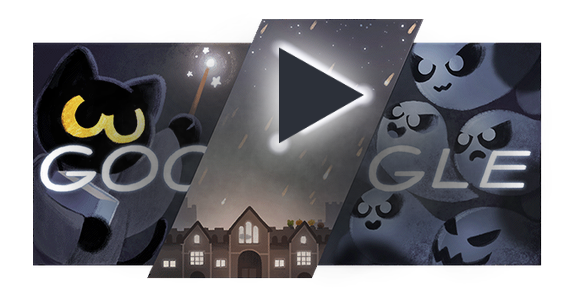
\includegraphics[width=0.6\textwidth]{archivos/doodle.png}
  \caption{Doodle Halloween 2016}
  \label{fig:doodle}
\end{figure}

\vspace{0.5cm}

En este juego seremos Momo, una gata cuyo \textbf{objetivo es recuperar el libro de hechizos mágicos} de su escuela que los espíritus han robado. Para ello, debemos enfrentarnos a ellos  \textbf{dibujando en la pantalla} con ayuda del ratón los  \textbf{símbolos} que llevan justo en la parte superior para derrotarlos, avanzar por las salas de la escuela y dar con el jefe. Si algún fantasma nos  \textbf{alcanza} perderemos una {vida} de un  \textbf{total de 5} y al quedarnos sin ellas acabará la partida. Además, cuanto más rápido y mejor realicemos los patrones de los enemigos conseguiremos acumular  \textbf{combos} que nos aumentarán la  \textbf{puntuación}.

\begin{figure}[htbp]
\centering
  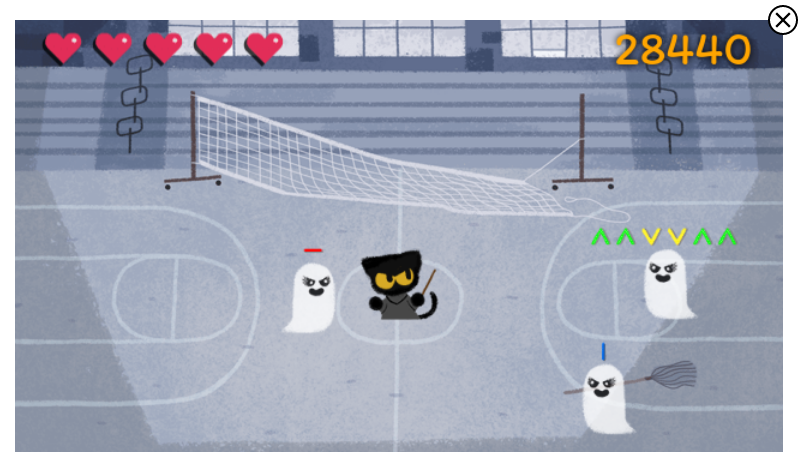
\includegraphics[width=0.6\textwidth]{archivos/juego.png}
  \caption{Cuarto nivel del juego, el gimnasio}
  \label{fig:halloweencat1}
\end{figure}

\vspace{0.5cm}

El juego consta de \textbf{5 niveles} más un nivel de \textbf{jefe final}. En cada nivel hemos de derrotar a una serie de fantasmas y a un jefe con un comportamiento \textbf{único y característico}. A medida que los niveles van avanzando la \textbf{dificultad aumenta}, pues la \textbf{velocidad} de los fantasmas es mayor y también empiezan a aparecer enemigos con \textbf{combinaciones de patrones más complejas y largas}.

\vspace{0.5cm}

Los tipos de patrones que nos podemos encontrar son:

\begin{itemize}
  \item \textbf{Línea vertical:} Por sí solo no tiene efecto diferente, puede combinarse con los demás.
  \item \textbf{Línea horizontal:} Por sí solo no tiene efecto diferente, puede combinarse con los demás.
  \item \textbf{Flecha hacia arriba ($\wedge$):} Por sí solo no tiene efecto diferente, puede combinarse con los demás.
  \item \textbf{Flecha hacia abajo ($\vee$):} Por sí solo no tiene efecto diferente, puede combinarse con los demás.
  \item \textbf{Rayo:} Este patrón es más fuerte que los anteriores, si lo dibujamos cuando hay varios enemigos en pantalla afectará a todos, quitándole un par de símbolos a cada enemigo. Puede combinarse con los demás
  \item \textbf{Corazón:} Aparece de vez en cuando siempre que no tengamos la vida a tope, si lo dibujamos conseguiremos recuperar una unidad de vida.
\end{itemize}

\vspace{0.5cm}

El \textbf{nivel del jefe final} es algo distinto a los demás ya que no sigue la estructura que estos mantenían. En este nivel deberemos derrotar primero a una serie de fantasmas y después dibujar una combinación de patrones muy larga que el jefe posee para hacerle daño antes de que nos alcance. Esto se deberá \textbf{repetir tres veces}, y por supuesto la velocidad y complejidad aumenta cuanto más cerca estemos de derrotarlo.

\begin{figure}[htbp]
\centering
  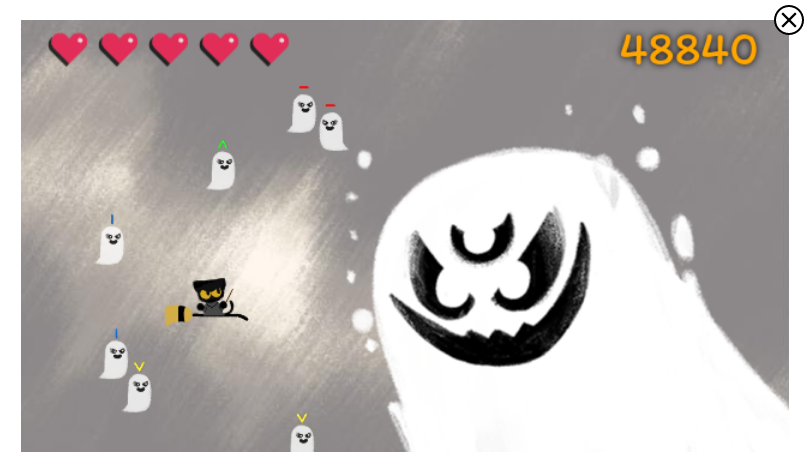
\includegraphics[width=0.6\textwidth]{archivos/jefe-horda.png}
  \caption{Primera fase del jefe donde aparecen enemigos.}
  \label{fig:jefe1}
\end{figure}

\clearpage

\begin{figure}[htbp]
\centering
  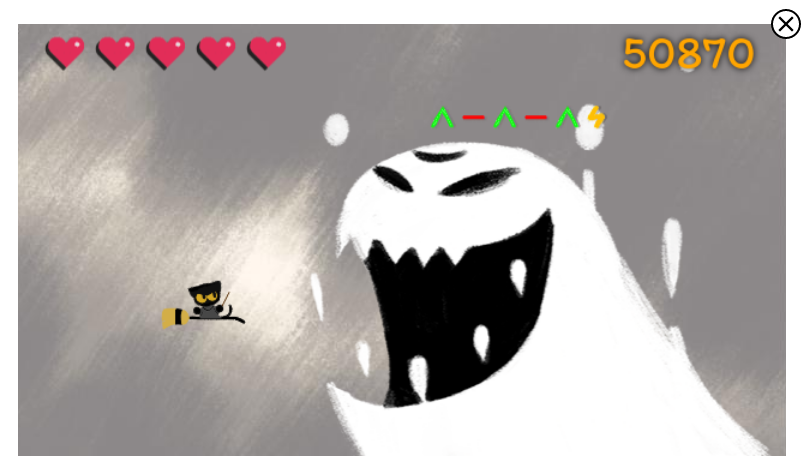
\includegraphics[width=0.6\textwidth]{archivos/jefe-ataque.png}
  \caption{Segunda fase del jefe donde le atacamos diréctamente}
  \label{fig:jefe2}
\end{figure}

\vspace{0.5cm}

Como ya se ha comentado, el jugador puede ir acumulando combos para mejorar su puntuación. Tanto si ganamos la partida como si la perdemos, podremos \textbf{compartir en las redes sociales nuestra puntuación}. Esto es una buena idea ya que permite que los usuarios compartan sus experiencias con otros y les inciten a jugar ya que aporta cierto factor de \textbf{competitividad}.

\begin{figure}[htbp]
\centering
  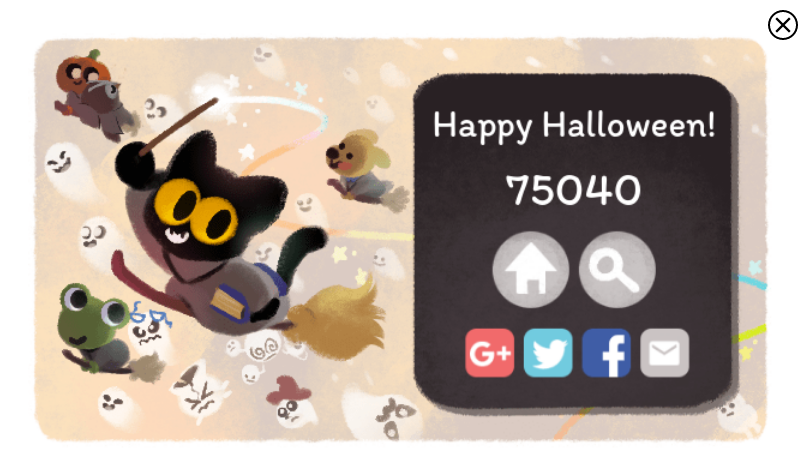
\includegraphics[width=0.6\textwidth]{archivos/pantalla-win.png}
  \caption{Pantalla que aparece al completar el juego}
  \label{fig:halloweenwin}
\end{figure}

\clearpage

\begin{figure}[htbp]
\centering
  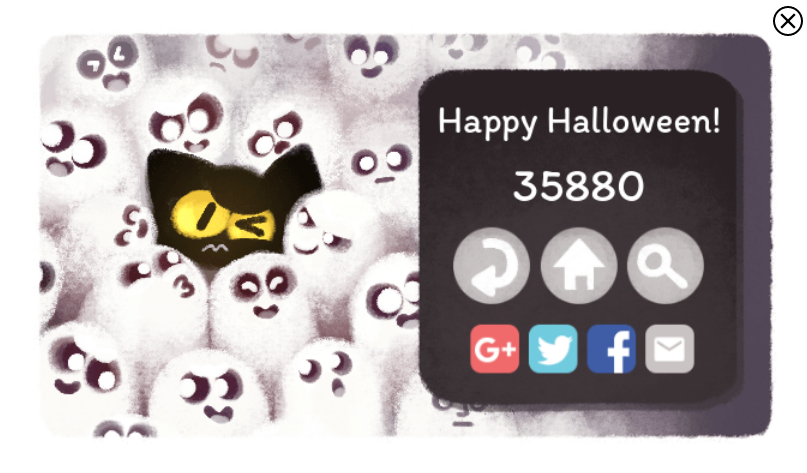
\includegraphics[width=0.6\textwidth]{archivos/pantalla-game-over.png}
  \caption{Pantalla que aparece al perder todas tus vidas.}
  \label{fig:halloweengo}
\end{figure}

Como curiosidad, el juego fue desarrollado por 4 grupos de aproximadamente 4 o 5 personas cada uno. Constaban de un grupo de arte, otro de producción, uno de ingenieros y uno de ``ayuda extra'' donde se realizaba la música.

\vspace{0.5cm}

Ahora bien, hemos elegido este juego como \textbf{principal referente} en cuanto a las \textbf{mecánicas}. Diseñaremos el juego de modo que la esencia y jugabilidad sean prácticamente las mismas. Creemos que un juego de estas características es algo sencillo pero que puede ser muy\textbf{ escalable}, facilitando el desarrollo por iteraciones. También es\textbf{ divertido} y un candidato perfecto para la NDS ya que parece estar hecho para jugarlo con una \textbf{pantalla táctil}.

\vspace{1cm}

\subsection{Una pausa con... Brain Training Ciencias}

Una pausa con... Brain Training o también conocido como Brain Age Express en América, se trata de una serie \textbf{tres juegos educacionales de resolver puzzles} desarrollados por Nintendo y publicados en el servicio \textbf{DSi Ware} de manera \textbf{gratuita} en 2009 en Europa.

\vspace{0.5cm}

Estos tres juegos se tratan de un \textbf{recopilatorio} de los puzzles que más les habían gustado a los jugadores de los \textbf{títulos previos} como Brain Training ¿Cuántos años tiene tu cerebro? y su secuela Más Brain Training para NDS. No obstante, le daban una vuelta de tuerca a estos puzzles haciéndolos \textbf{más desafiantes y divertidos}, incluso integraban el uso de la \textbf{cámara} al ser un proyecto para DSi.

\clearpage

\begin{figure}[htbp]
\centering
  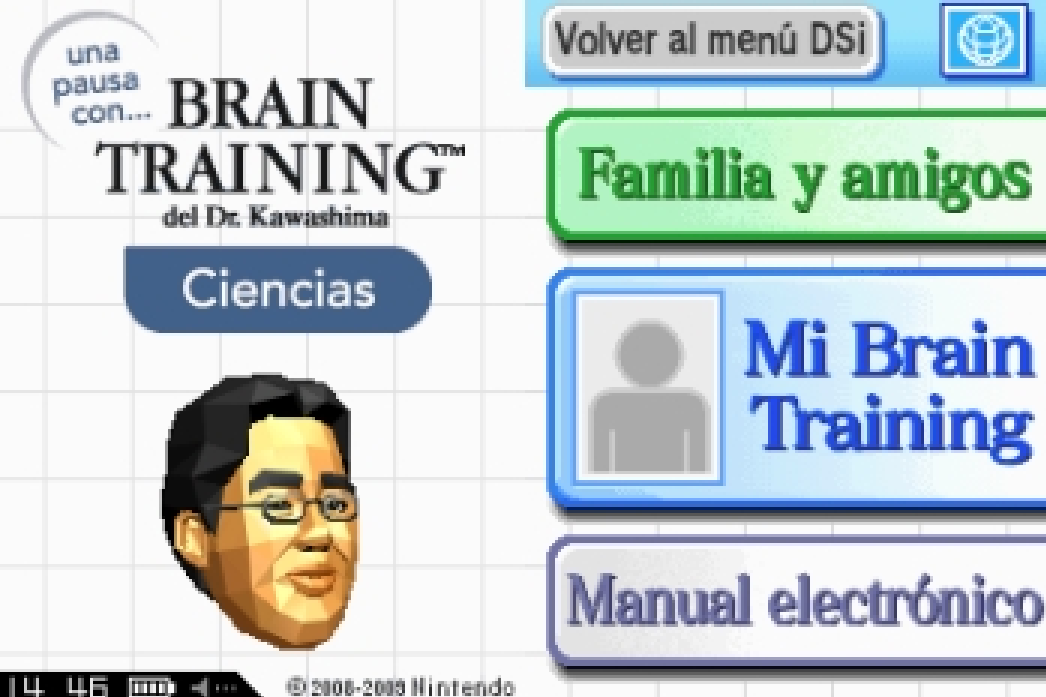
\includegraphics[width=0.6\textwidth]{archivos/brain.png}
  \caption{Menú principal de Una pausa con... Brain Training Ciencias}
  \textbf{Fuente:} \href{https://www.nintendo.es/Juegos/Nintendo-DSiWare/Una-pausa-con-Brain-Training-Ciencias-261960.html}{Nintendo}
  \label{fig:sbraintraining1}
\end{figure}

\vspace{0.5cm}

Todos los títulos de esta saga tienen un mismo \textbf{objetivo}: jugar unos minutos \textbf{diariamente} a una serie de puzzles de \textbf{cálculo}, \textbf{memorización de imágenes o datos} e incluso ejercicios de \textbf{ortografía y lectura}, con el fin de \textbf{ejercitar el cerebro}. No obstante, también proporciona la opción de jugar a dichos puzzles de manera individual e incluso tienen un \textbf{modo sudoku}.

\vspace{0.5cm}

Volviendo a nuestro referente, como hemos comentado se trata de una serie de tres juegos divididos en \textbf{categorías} de \textbf{ciencias, letras y sudoku}. Por una razón que no se hizo oficial, Nintendo quitó del servicio de DSi Ware la edición de sudokus, mientras que las otras dos se mantuvieron e incluso venían preinstaladas en las NDSi americanas. En concreto nos vamos a centrar en la edición de ciencia, pues hay un puzzle particular que tiene bastante relación con nuestro juego: el \textbf{Suma y Sigue}.

\begin{figure}[htbp]
\centering
  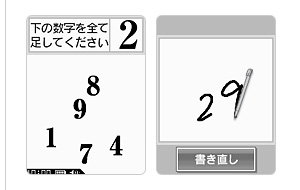
\includegraphics[width=0.6\textwidth]{archivos/brain-sumtotaled1.jpg}
  \caption{Minijuego Suma y Sigue en su modo normal}
    \textbf{Fuente:} \href{https://www.nintendo.co.jp/ds/dsiware/kndjknrj/training2/index.html}{Nintendo}
  \label{fig:sumtotaled1}
\end{figure}

\vspace{0.5cm}

En este minijuego debemos realizar la \textbf{suma} de los \textbf{números} que veremos esparcidos por la pantalla y escribir el resultado en la pantalla táctil \textbf{lo antes posible}. Posee \textbf{dos modos de juego}, uno normal que es el que acabamos de explicar y otro \textbf{arcade}, el que nos interesa. El objetivo del modo arcade es exactamente el mismo, realizar la suma de números, pero con el añadido de que los números ahora no están colocados aleatoriamente en la pantalla, si no forman el cuerpo de un \textbf{enemigo} que se va acercando hacia el jugador para quitarle vida. Este modo otorga un factor más \textbf{desafiante} al juego ya que en el primer modo si fallamos la operación obtendremos peor resultado en la prueba, mientras que en el modo arcade al tener un máximo de tres vidas y ver cómo los enemigos se acercan provoca \textbf{presión} en el jugador.

\begin{figure}[htbp]
\centering
  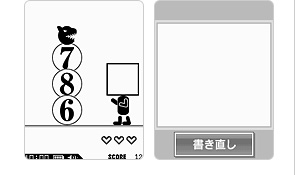
\includegraphics[width=0.6\textwidth]{archivos/brain-sumtotaled2.jpg}
  \caption{Minijuego Suma y Sigue en su modo arcade}
  \textbf{Fuente:} \href{https://www.nintendo.co.jp/ds/dsiware/kndjknrj/training2/index.html}{Nintendo}
  \label{fig:sumtotaled2}
\end{figure}

La razón por la que se ha elegido este minijuego como referente es por poseer algunas \textbf{características adicionales} que Magic Cat Academy no posee con respecto a los enemigos y que podrían aportar más diversión si se \textbf{mezclan}. Por ejemplo, los enemigos a veces se esconden haciendo que \textbf{no se puedan ver} parte de sus números, también dichos números \textbf{se mueven} alrededor del cuerpo de dicho enemigo, haciendo que sea más complicado realizar el cáclulo.

\vspace{1cm}

\subsection{Lost Magic}

Lost Magic es un juego \textbf{RPG} de \textbf{estrategia en tiempo real} desarrollado por \textbf{Taito} para NDS y publicado en 2006.

\vspace{0.5cm}

En este juego seremos el mago Isaac, cuyo padre le otorga una varita poderosa con la cual lanzar hechizos potentes. Isaac deberá avanzar en la historia \textbf{derrotando unos enemigos} en un \textbf{tiempo determinado}. Para ello, puede moverse por el mapa y al encontrarse a un enemigo mantener pulsado  el botón L, esto abrirá un menú donde puede invocar hechizos dibujándolos en la pantalla táctil, siempre y cuando antes los haya aprendido. Una vez dibujado el hechizo simplemente debe tocar  a qué enemigo desea lanzárselo y cuanto \textbf{más rápido y mejor lo dibujemos}, más \textbf{efectivo} será. Por último, para poder realizar estos hechizos necesita \textbf{poder mágico}, cada vez que realice uno este disminuirá y para que vuelva a aumentar simplemente debemos esperar unos segundos.

\begin{figure}[htbp]
\centering
  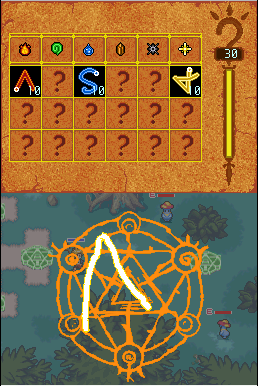
\includegraphics[width=0.4\textwidth]{archivos/lostmagic2.png}
  \caption{Principal mecánica del Lost Magic. Arriba vemos los conjuros aprendidos y abajo en la pantalla táctil podemos dibujarlos.}
  \label{fig:lostmagic1}
\end{figure}

\vspace{0.5cm}

Como muchos RPGs, el jugador también irá subiendo de nivel, mejorando sus características mágicas, y obteniendo objetos.

\clearpage

\begin{figure}[htbp]
\centering
  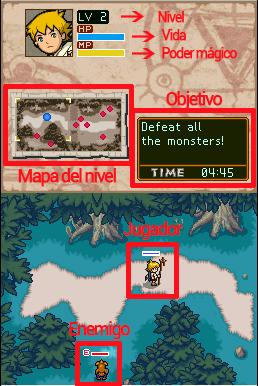
\includegraphics[width=0.4\textwidth]{archivos/lostmagic1.png}
  \caption{Elementos del juego típicos de un RPG.}
  \label{fig:lostmagic2}
\end{figure}

\vspace{0.5cm}

La razón por la que hemos elegido este juego es por estudiar cómo \textbf{implementa el dibujado en tiempo real de los patrones} de hechizos en la pantalla de la NDS y el \textbf{reconocimiento} de estos. Al tratarse de un juego para la \textbf{misma consola} para la que estamos desarrollando y estar desarrollado por una gran empresa como es Taito, podemos hacernos una idea del \textbf{resultado} que podríamos obtener y las limitaciones que existen.

\vspace{1cm}

\subsection{Wario Ware: Touched!}

Wario Ware: Touched!  es un juego basado en \textbf{minijuegos} de la saga Wario Ware que \textbf{Nintendo} desarrolló para la NDS en 2004.

\vspace{0.5cm}

En este juego tendremos distintos \textbf{niveles representados por personajes} tales como Wario, Mona, Kat y Ana, Ashley... En \textbf{cada nivel} debemos pasarnos una \textbf{serie de minijuegos muy cortos en un tiempo determinado} (unos 15 segundos) que suelen ser de dibujar algo en la pantalla táctil, soplar al micrófono, etc. Si no lo logramos, \textbf{perderemos una vida}, lo cual es muy importante pues al pasarnos una serie de minijuegos llegará el \textbf{minijuego de final de nivel} que deberemos completar para completarlo.

\clearpage


\begin{figure}[htbp]
\centering
  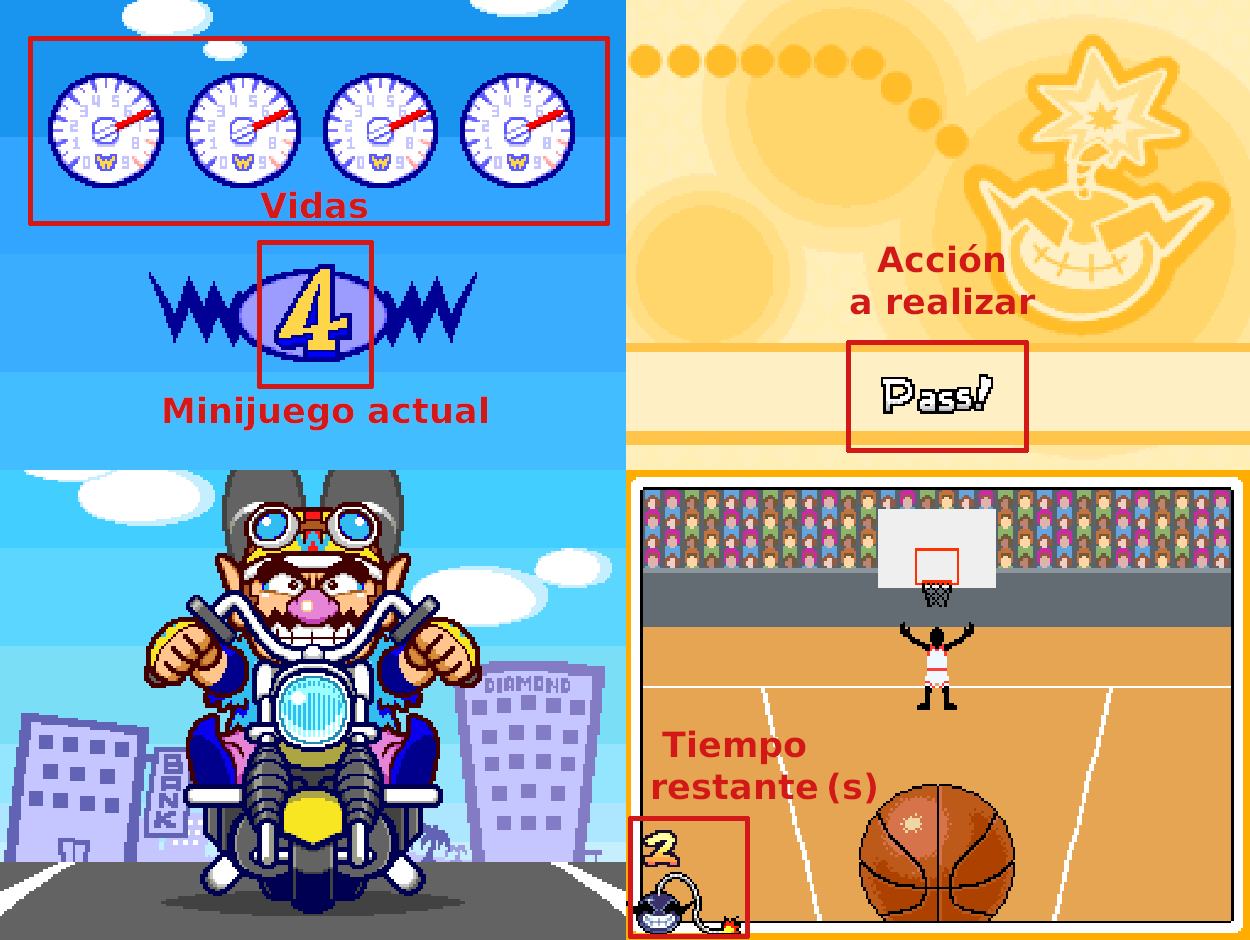
\includegraphics[width=0.6\textwidth]{archivos/wario_ware_level.png}
  \caption{Pantalla de cambio entre minujuegos y minujuego específico de Wario Ware: Touched!.}
  \label{fig:wario_ware_level}
\end{figure}

\vspace{0.5cm}

La razón de escoger este juego como referente es la misma que la de Lost Magic. Me gustaría estudiar cómo es capaz de \textbf{dibujar en tiempo real trazados del usuario} así como gran cantidad de \textit{sprites} y fondos en pantalla que aparecen y desaparecen en cuestión de segundos, \textbf{optimizando así los recursos de la consola}. También, personalmente me gusta mucho el \textbf{estilo del arte} en los \textit{sprites} y diseño de personajes ya que son bastante carismáticos y únicos, y en cierto modo me gustaría inspirarme en ello para poder crear los de este proyecto.

\vspace{1cm}
